\chapter{Demystifying Neurodivergence via Score Estimators }
\label{ch:localizing}

Given the success of MSMA for anomaly detection on benchmark experiments, we will now explore whether this methodology allows for any new \textit{scientific} insights.
Assuming the underlying model has learned rich information about the data, can it help us uncover additional knowledge about our dataset? I will try to answer that question by focusing on a narrow task: detecting neuroatypicalities from structural MRIs of adolescent brains.
% The task was chosen such that \textit{if} a novel insight is derived, it may be of direct use to the medical research community.

Atypically developing children are diagnosed through clinical assessments that measure behavioral response. While effective in diagnosis, behavioral assessments do not provide any insight into the differences in brain morphometry of the neurodivergent cohort. Existing analyses primarily look at group wise differences of brain features (such as region volumes) between cohorts~\cite{giraultNeurodevelopmentAutismInfancy2020,hamnerPediatricBrainDevelopment2018}, or correlations of said features with a behavioral assessment~\cite{shenSubcorticalBrainDevelopment2022,brainsci12040439}. These analyses fail to produce specific causal relationships between the brain regions and the neurodivergence, as they mainly focus on correlational evidence.
Furthermore, the researchers introduce additional biases when they select regions of interest (ROIs) to be studied using their preconceived notions about the disease.

Herein lies the opportunity for a data-driven methodology to uncover atypically developing ROIs that are reflected in the data but, may be underexplored in the existing  literature. One can task a model to identify subpopulations that deviate from the typical (via outlier detection), and subsequently highlight the brain ROIs shared across the subpopulations (via localization).  MSMA, combined with its localization augmentation, naturally allows for such data exploration. This chapter outlines a process through which MSMA was utilized to derive insights about brain MRI data.

\section{A Hypothesis Generating Tool}

The previous chapters have demonstrated MSMA's anomaly detection capabilities. At the heart of MSMA is the score-norm vector, which describes a space in which the outliers become separable from the inliers. How can one explore this space to gain further insights into the data?

We can assume that a user exploring the outputs of MSMA will be looking to answer a set of research questions. Examples of the questions may be:
\begin{itemize}
    \item Do any subpopulations cluster in the score-norm space?
    \item Can we identify atypical input features (such as brain ROIs)  that are shared among samples within a cluster?
    \item Do subpopulations in the score-norm space correlate with any external measurements (such as behavioral assessments)?
\end{itemize}

To answer such questions, one needs to be able to link multiple sources of data: the score-norm space, the localization heatmaps, and existing metadata associated with each sample. I posit to use an interactive visualization to facilitate such a task.
Using the visualization the user should be able to observe how samples are distributed in the score-norm space. Additional views can show the aggregated localization heatmaps for each cluster, as well as metadata such as behavioural scores.

% The visualization will also display an aggregate of anomaly scores across brain ROIs. The goal of the visualization is to make the results interpretable by a medically informed audience. By using standardized brain parcellation schemes, the visualization should enable the user to identify the most anomalous ROIs for the population of interest, and refer to the medical literature for further analysis.

\section{Exploring a High-Dimensional Space}

It is often desirable to visualize data for the purposes of exploratory research. This poses a problem if we want to visualize the space of score-norms (as a 2D image). While the score-norms are much lower in dimensionality compared to the high resolution MRIs they are derived from, each score-norm vector is still multidimensional. For reference, all of the experiments in this chapter use $L=20$ scales, resulting in a 20-dimensional vector for each sample. One has to utilize a dimensionality reduction algorithm to reduce the space into two or three dimensions so that the points may be plotted on a screen.

This section will briefly go over dimensionality reduction algorithms and why they may not be appropriate for our analysis as they can introduce spurious clusters in the visualization. Instead, I will be advocating the use of the Self-Organizing Map (SOM)~\cite{kohonen1990self}  to visualize my data and will discuss its advantages.


\subsection*{Common Dimensionality Reduction Algorithms}

Conventionally, researchers have used PCA\tempcite{PCA} to select the most important components to display. While this technique is fast and well understood, it has the downside of only capturing linear subspaces as it will select orthogonal components of highest variation. Recently, two other techniques have gained popularity as methods to visualize high dimensional non linear data: t-SNE and UMAP.  

% \subsection*{A Brief Discussion on t-SNE and UMAP}

t-SNE (t-distributed Stochastic Neighbor Embeddings) defines the relative distance between two points as a conditional probability. It uses an optimization process to determine a low-dimensional embedding such that the relative distance between each point in the low-dimensional space matches the distance in the high-dimensional space (using the Kullback-Leibler Divergence between the pairwise conditional probability distribution).

UMAP (Uniform Manifold Approximation and Projection) computes the low-dimensional embedding in two stages. First, it constructs a weighted graph of the k-nearest neighbours (the number of neighbors being a hyperparameter). The weights of the graphs represent probability distributions. In the second stage, it uses an iterative procedure to pull the neighbors in the graph closer together in the low-dimensional space. Additionally, it applies a repulsive force between all non-neighbours in the graph, pushing them away in the low-dimensional space. Generally, UMAP is considered to have superior runtime performance compared to t-SNE~\cite{mcinnes2020umap}

\subsection*{t-SNE and UMAP Need Not Reflect the Data}
% why are they not optimal for the task?

Both t-SNE and UMAP aim to find a low-dimensional space that reflects the distances in the original space. However, the resulting low-dimensional space is highly dependant on the hyperparameters. These hyperparameters (associated with the size of the neighbourhood considered) produce a trade-off between the preservation of local structure and preservation of global structure. Often, the algorithms are unable to preserve both~\cite{pacmap}. If local structure is emphasized, the algorithms produce spurious clusters, making their results untrustworthy. Conversely, if global structure is emphasized, the algorithms tend to produce large homogenous blobs, and fail to distinguish any underlying patterns~\cite{leiQuantifyingImpactUninformative2023}.
% This can have the unfortunate effect of the practitioner tweaking the hyperparameters until the algorithm's output plots that coincide with the practitioner's existing beliefs.


\subsection*{Self Organizing Maps as an Alternative}

The Self-Organizing Map, also known as Kohonen Networks, ~\cite{kohonen1990self} produces a two-dimensional grid-like map such that each cell on the map corresponds to a location in the data-space. Nearby cell locations on the grid are closer in the data-space compared to distal cell locations. A cell is commonly also referred to as a 'neuron'.

During training, the method randomly initializes a grid of neurons (cells). Note that the weight vector corresponding to each neuron resides in the data-space. For each data sample we find the closest neuron to the current point. This is referred to as the Best Matching Unit (BMU). The BMU's weights are updated to be closer to the data point. Additionally, the neighboring neurons (in the \textit{grid-space}) are also updated. The latter step is crucial to preserve the topological structure of the data. This procedure is repeated for a pre-defined number of iterations. Most online packages implement the batch-learning algorithm described by~\cite{kinouchi2002quick}. The authors improve convergence by initializing the neurons using the first two eigenvectors computed from the data, and by modifying learning objective to use the full dataset in each weight update rather than a minibatch as in the original algorithm.  I will be using the latter training algorithm.

\subsection*{SOMs Circumvent Dimensionality Reduction}

Note that SOMs operate directly in the high-dimensional data space, computing distances between the data points and the neuron prototypes in this original space. The topological constraint on the grid of neurons mainly facilitates the visual organization. This is in contrast to t-SNE and UMAP, which first project the data into a low-dimensional space, where distance computations may not accurately reflect the true distances in the high-dimensional space. As a result, SOMs can better preserve the structure and relationships within the data, reducing the risk of distortions introduced by dimensionality reduction.

\subsection*{SOMs Identify Prototypes}
It is helpful to think of SOM as a vector quantization algorithm with a spatial constraint on the codebook of vectors. Thus, each neuron can be interpreted as a prototype in the data-space. The grid-like structure of SOMs provides a natural way to organize these data prototypes. The relative positions of the neurons on the grid reflect their similarities. This spatial organization can aid in identifying patterns, clusters, or relationships within the data that may not be immediately apparent from a scatter plot produced by techniques like t-SNE or UMAP.

To elucidate how one can use SOM to gain insights about the data, recall that each sample is assigned to a single neuron (the sample's BMU). If class labels are available, we can tally up the labels of all the samples that are assigned to a given neuron. The maximally matching label can then be computed for each neuron. This label is often overlayed on top of the map visualization to quickly associate the prototype with a population.
[EXAMPLE in fig]


% One can go further and analyze the hsitogram
% \subsection*{SOM vs tsne for clustering}

% \section{Feasibility Experiments on Benchmark Datasets }

\section{Case Study: Detecting Brain ROIs involved in Down Syndrome}

Down Syndrome (DS) is one of the most common neurodevelopmental disorder, occurring at a rate of ~1/700 live births~\cite{parker2010updated}. Studies have revealed large deviations from typical development in brain structure of children with DS, with the most pronounced deviation in the total brain volume (TBV). Further, when TBV is accounted for, studies have revealed deviations in specific regions of the brain such as the temporal lobe, cerebellum, and hippocampus~\cite{hamnerPediatricBrainDevelopment2018}. However, there remains a push for developing focused research to elucidate the nature of DS neuroanatomic phenotypes~\cite{hamnerPediatricBrainDevelopment2018}.

This case study aims to uncover brain ROIs that are associated with DS, using learned score-estimates. It will incorporate MSMA, SOMs, and Spatial-MSMA to provide a cohesive analysis of structural brain MRIs belonging to a DS cohort.

The case study will be answering the following research questions:
    - Do the ROI anomaly scores \textit{correlate} with any behavior assessment?
 
    - Can Spatial-MSMA isolate brain ROIs relevant to the prototype?
 
    - Does the score-norm space produced by MSMA capture any neuroanatomic phenotype(s) pertinent to DS ?
 
	% - Does Spatial-MSMA highlight brain ROIs that are \textit{known} in the existing research?

	% - Does Spatial-MSMA highlight brain ROIs that are \textit{novel}?
 



\subsection*{Data and Methodology}
 % As a first pass, all images with low automated QC scores were removed. --- > move this into appendix or ch:local
 
As in Chapter~\ref{ch:localizing}, we will be using samples from the ABCD and HCPD study as our reference inliers. I will denote this as ABCD-HCPD. This cohort was preprocessed to remove any outlying samples. To keep the inlier cohort as nominal as possible, we used the Child Behavior Checklist (CBCL)~\tempcite{CBCL} scores as our filtering mechanism. This checklist assesses the behavior and emotional competencies of children. Children with behavioral problems tend to score high on this test. For our analysis, all children that scored above a t-score of 66 ($\tilde~95$-th percentile) in the summary scores as well as \textit{any} of the subscores were removed. Note that this is more conservative than only using the summary scales.

Our testing population is retrieved from the Infant Brain Imaging Study (IBIS) study~\tempcite{IBIS}. The goal of the study is to investigate brains starting from infancy and following up at later ages. The study is primarily focused on investigating Autism Spectrum Disorder (ASD) but has also gathered data for Down's Syndrome.This section will be looking at school-age scans as they best overlap with the ages in the ABCD study. IBIS uses a protocol to determine typically developing children, as a means of obtaining a control population. This control sample have to be non-ASD as well as low-likelihood (no sibling with ASD). The control population was further filtered using Autism Diagnostic Observation Schedule (ADOS)~\tempcite{ADOS} scores. Specifically, we removed samples that had an ADOS score above 2.

A 3D diffusion model was trained on the ABCD-HCPD dataset. At inference time, the diffusion model was used to obtain score norms for the IBIS data as well as a held out test-set of ABCD-HCPD. A Spatial-MSMA model was also trained on the score-norms of the ABCD-HCPD samples. This allowed us to obtain the voxel-wise anomaly scores for each test sample. These anomaly scores were then averaged according to ROIs retrieved from the AAL atlas~\cite{ROLLS2020116189}. Addiitonally, a SOM was trained on the inlier score-norms from all three studies. 

% Additionally, the CSF was also included in the analysis

\subsection*{Does Spatial-MSMA Capture Relevant Brain ROIs?}


% \subsection*{Self-Organizing Maps of MSMA reveal a DS Prototype}
\subsection*{Does MSMA reveal a DS Prototype?}

% Does MSMA capture
This research question can be answered by analyzing the outputs of a SOM trained on the score-norm space computed via MSMA. 

Recall that each sample is matched with one BMU, represented as a cell in the grid. Let us consider the BMU with the most matches for a particular cohort. I will denote this BMU as the Maximal-Prototype. 

In~\figref{fig:som-abcd}, we can clearly observe a Maximal-Prototype for the DS cohort. Out of 28 DS cases, 16 match this prototype. Furthermore, 12 out of the matching 16 are female. This points to a female-dominant DS phenotype.

- distribution of ROI scores
 - roi scores are percentiles wrt abcd-hcpd
- how do these ROI scores differ from other DS?
- 


\subsection*{Prototype Consistently Detected Across Experiments}

When using a data exploration tool such as SOM for producing scientific insights, it is crucial to delineate true correlations that exist in the data and spurious correlations that may be caused by random variations in the algorithm. Therefore, to increase our confidence in the findings, it is helpful to analyze the stability of the algorithm across runs with different hyperparameters. If the algorithm outputs consistent results, then one can have more confidence when interpreting the results.

SOM has two main hyperparameters: the number of rows, and the number of columns in the grid. We can assess whether SOM consistently finds the same Maximal-Prototype for DS.

[FIG] shows a heatmap of the number of samples that matched the Maximal-Prototype in each experiment. We can observe that the number of matches remain consistent across different hyperparameters. Smaller grid sizes will have the most matches as there are only a few candidate prototypes. Large grid sizes will cause a more refined binning, resulting in multiple prototypes which are relatively close to one another. We can observe large ''bands" of stability in the middle regions.

Further analysis revealed that each band captures the \textit{same} samples as well as having a perfect overlap with the one before it. For instance, the set of experiments that produced a 16-sample prototype not only captured the same 16 samples within the set of experiments, but also the same samples that were capture by the 15-sample prototype. This indicates that SOM is capturing a true sub-population of DS samples in the score-norm space rather than matching at random.



% Another interesting point to note, is the specificity of this prototype. Only 17 (non-inlier) samples matched with this prototype


\begin{figure}[tbhp]
\centering
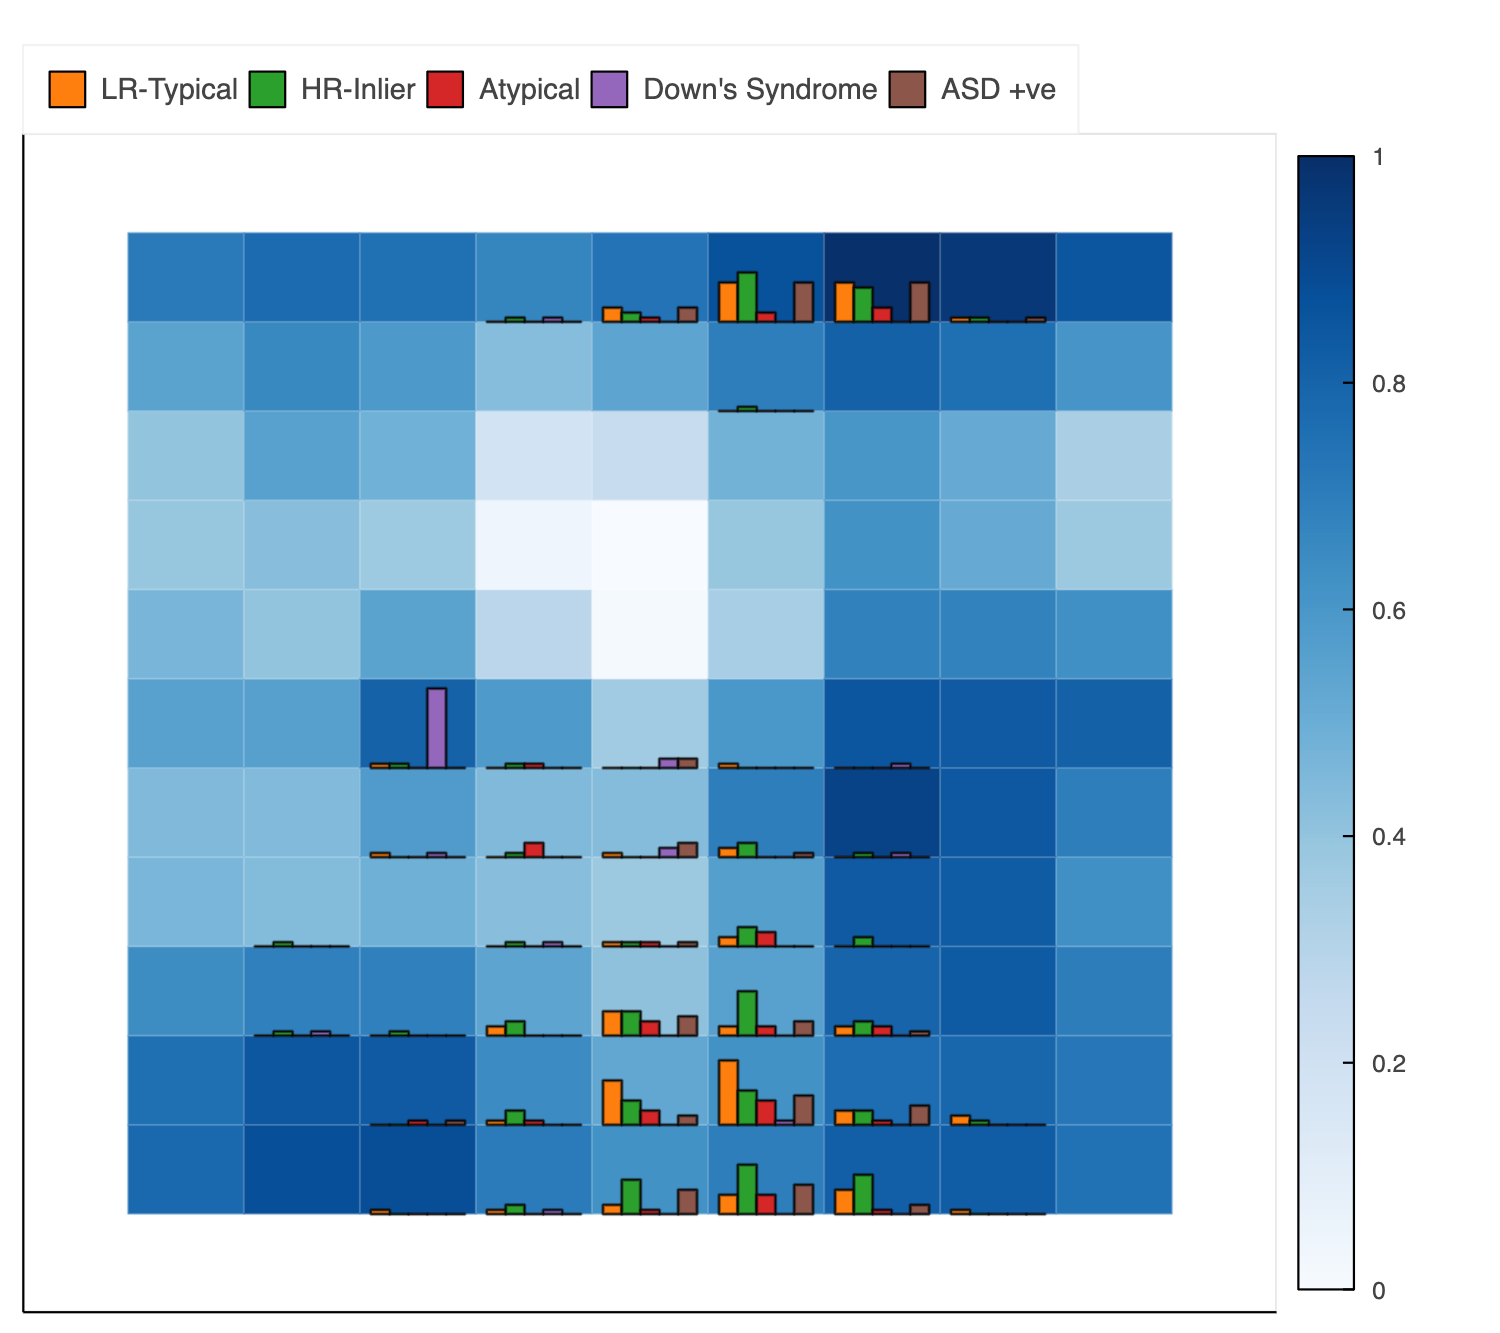
\includegraphics[width=\linewidth]{figures/somgrid.png}
\caption{A Self-Organizing Map trained on score-norms of brain MRIs of typically developing children. Overlayed are the distributions of all cohorts matched to each cell in the grid.}
\label{fig:som-abcd}
\end{figure}





% vector qunatization flavored
% we are determining codebooks
% each protoype resides in the data space
